

\tikzset{every picture/.style={line width=0.75pt}} %set default line width to 0.75pt        

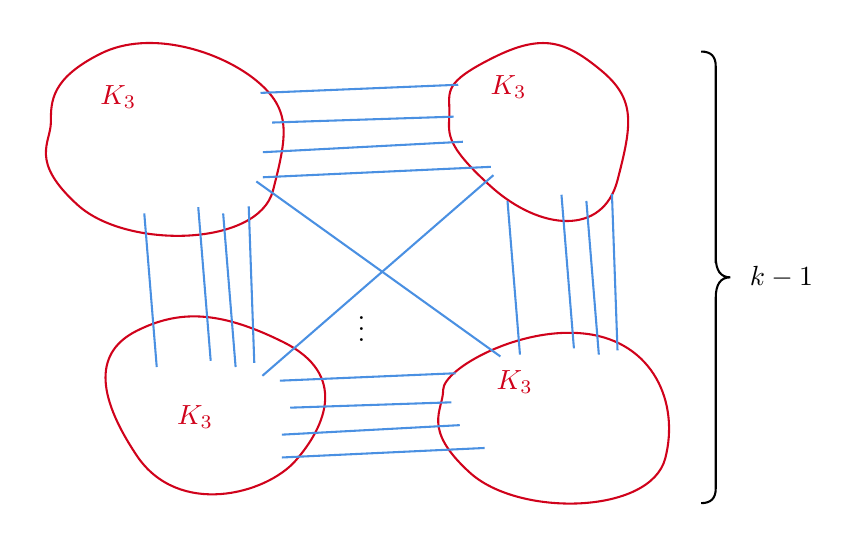
\begin{tikzpicture}[x=0.75pt,y=0.75pt,yscale=-1,xscale=1]
	%uncomment if require: \path (0,300); %set diagram left start at 0, and has height of 300
	
	%Shape: Polygon Curved [id:ds09085431314278214] 
	\draw  [color={rgb, 255:red, 208; green, 2; blue, 27 }  ,draw opacity=1 ] (45.68,54.42) .. controls (69.68,42.42) and (103.68,53.42) .. (120.68,67.42) .. controls (137.68,81.42) and (135.68,93.42) .. (128.68,120.42) .. controls (121.68,147.42) and (58.37,148.83) .. (34.68,127.42) .. controls (11,106) and (21.68,97.42) .. (21.68,87.42) .. controls (21.68,77.42) and (21.68,66.42) .. (45.68,54.42) -- cycle ;
	%Shape: Polygon Curved [id:ds8870410137343234] 
	\draw  [color={rgb, 255:red, 208; green, 2; blue, 27 }  ,draw opacity=1 ] (234.68,56.42) .. controls (258.68,44.42) and (269.68,48.42) .. (286.68,62.42) .. controls (303.68,76.42) and (301.68,88.42) .. (294.68,115.42) .. controls (287.68,142.42) and (257.37,139.83) .. (233.68,118.42) .. controls (210,97) and (213.68,92.42) .. (213.68,82.42) .. controls (213.68,72.42) and (210.68,68.42) .. (234.68,56.42) -- cycle ;
	%Shape: Polygon Curved [id:ds16158191908791397] 
	\draw  [color={rgb, 255:red, 208; green, 2; blue, 27 }  ,draw opacity=1 ] (63,188) .. controls (83,178) and (102.37,177.83) .. (133.68,193.42) .. controls (165,209) and (154,234) .. (139.68,250.42) .. controls (125.37,266.83) and (83,278) .. (63,248) .. controls (43,218) and (43,198) .. (63,188) -- cycle ;
	%Shape: Polygon Curved [id:ds6987345702479908] 
	\draw  [color={rgb, 255:red, 208; green, 2; blue, 27 }  ,draw opacity=1 ] (279.68,189.42) .. controls (311.68,193.42) and (324.68,222.42) .. (317.68,249.42) .. controls (310.68,276.42) and (247.37,277.83) .. (223.68,256.42) .. controls (200,235) and (210.68,226.42) .. (210.68,216.42) .. controls (210.68,206.42) and (247.68,185.42) .. (279.68,189.42) -- cycle ;
	%Shape: Brace [id:dp3001695353726017] 
	\draw   (335,271) .. controls (339.67,271) and (342,268.67) .. (342,264) -- (342,172.21) .. controls (342,165.54) and (344.33,162.21) .. (349,162.21) .. controls (344.33,162.21) and (342,158.88) .. (342,152.21)(342,155.21) -- (342,60.42) .. controls (342,55.75) and (339.67,53.42) .. (335,53.42) ;
	%Straight Lines [id:da8439459671619836] 
	\draw [color={rgb, 255:red, 74; green, 144; blue, 226 }  ,draw opacity=1 ]   (122.68,73.35) -- (217.94,69.42) ;
	%Straight Lines [id:da4840228989658659] 
	\draw [color={rgb, 255:red, 74; green, 144; blue, 226 }  ,draw opacity=1 ]   (128.31,87.63) -- (215.69,84.8) ;
	%Straight Lines [id:da2850505043333227] 
	\draw [color={rgb, 255:red, 74; green, 144; blue, 226 }  ,draw opacity=1 ]   (123.81,101.92) -- (220.19,96.88) ;
	%Straight Lines [id:da33929995101795196] 
	\draw [color={rgb, 255:red, 74; green, 144; blue, 226 }  ,draw opacity=1 ]   (123.81,114) -- (233.68,108.97) ;
	%Straight Lines [id:da9701949837269326] 
	\draw [color={rgb, 255:red, 74; green, 144; blue, 226 }  ,draw opacity=1 ]   (292,122) -- (294.68,197.42) ;
	%Straight Lines [id:da33173345207460336] 
	\draw [color={rgb, 255:red, 74; green, 144; blue, 226 }  ,draw opacity=1 ]   (241.68,125.42) -- (247.68,199.42) ;
	%Straight Lines [id:da7738376025469385] 
	\draw [color={rgb, 255:red, 74; green, 144; blue, 226 }  ,draw opacity=1 ]   (267.68,122.42) -- (273.68,196.42) ;
	%Straight Lines [id:da8778403311147553] 
	\draw [color={rgb, 255:red, 74; green, 144; blue, 226 }  ,draw opacity=1 ]   (279.68,125.42) -- (285.68,199.42) ;
	%Straight Lines [id:da9164505964805534] 
	\draw [color={rgb, 255:red, 74; green, 144; blue, 226 }  ,draw opacity=1 ]   (117,128) -- (119.68,203.42) ;
	%Straight Lines [id:da26272014242408237] 
	\draw [color={rgb, 255:red, 74; green, 144; blue, 226 }  ,draw opacity=1 ]   (66.68,131.42) -- (72.68,205.42) ;
	%Straight Lines [id:da47637448468384713] 
	\draw [color={rgb, 255:red, 74; green, 144; blue, 226 }  ,draw opacity=1 ]   (92.68,128.42) -- (98.68,202.42) ;
	%Straight Lines [id:da8366813568912879] 
	\draw [color={rgb, 255:red, 74; green, 144; blue, 226 }  ,draw opacity=1 ]   (104.68,131.42) -- (110.68,205.42) ;
	%Straight Lines [id:da5949105316211332] 
	\draw [color={rgb, 255:red, 74; green, 144; blue, 226 }  ,draw opacity=1 ]   (132,212) -- (216.68,208.42) ;
	%Straight Lines [id:da921463181820533] 
	\draw [color={rgb, 255:red, 74; green, 144; blue, 226 }  ,draw opacity=1 ]   (137,225) -- (214.68,222.42) ;
	%Straight Lines [id:da6617621009937191] 
	\draw [color={rgb, 255:red, 74; green, 144; blue, 226 }  ,draw opacity=1 ]   (133,238) -- (218.68,233.42) ;
	%Straight Lines [id:da4522991409867132] 
	\draw [color={rgb, 255:red, 74; green, 144; blue, 226 }  ,draw opacity=1 ]   (133,249) -- (230.68,244.42) ;
	%Straight Lines [id:da3448517677052281] 
	\draw [color={rgb, 255:red, 74; green, 144; blue, 226 }  ,draw opacity=1 ]   (120.67,116) -- (238.24,200.32) ;
	%Straight Lines [id:da3065278920610677] 
	\draw [color={rgb, 255:red, 74; green, 144; blue, 226 }  ,draw opacity=1 ]   (234.91,112.98) -- (123.58,209.65) ;
	
	% Text Node
	\draw (168,171.4) node [anchor=north west][inner sep=0.75pt]    {$\vdots $};
	% Text Node
	\draw (357,155.4) node [anchor=north west][inner sep=0.75pt]    {$k-1$};
	% Text Node
	\draw (44,68.4) node [anchor=north west][inner sep=0.75pt]  [color={rgb, 255:red, 208; green, 2; blue, 27 }  ,opacity=1 ]  {$K_{3}$};
	% Text Node
	\draw (232,63.4) node [anchor=north west][inner sep=0.75pt]  [color={rgb, 255:red, 208; green, 2; blue, 27 }  ,opacity=1 ]  {$K_{3}$};
	% Text Node
	\draw (81,222.4) node [anchor=north west][inner sep=0.75pt]  [color={rgb, 255:red, 208; green, 2; blue, 27 }  ,opacity=1 ]  {$K_{3}$};
	% Text Node
	\draw (235,205.4) node [anchor=north west][inner sep=0.75pt]  [color={rgb, 255:red, 208; green, 2; blue, 27 }  ,opacity=1 ]  {$K_{3}$};
	
	
\end{tikzpicture}